\chapter{Ressources}
  \section{Modèles AADL}
  \label{ann:aadl}

\lstdefinelanguage{aadl}{
  keywords={package, public, with, system, implementation, extends, end,
    subcomponents, connections, properties, reference, applies},
  keywordstyle=\bfseries,
  comment=[l]{--},
  commentstyle=\color{purple}
}

\lstset{
  language=aadl,
  backgroundcolor=\color{lightgray},
  basicstyle=\footnotesize\ttfamily,
  frame=single,
  rulecolor=\color{black},
  title={Vue globale du système.}
}

\begin{lstlisting}
package Demonstrator
public
 with Common::Buses;
 with NXT::Systems;
 with NXT::Devices;
 with Arduino::Systems; 
 with Arduino::Devices;
 
 system Demonstrator
 end Demonstrator;
 
 system implementation Demonstrator.Impl
 subcomponents
  NXT             : system NXT::Systems::NXT_System.Impl;
  Distance_Sensor : device NXT::Devices::DIST_Nx.v3;
  Wheel_Motor     : device NXT::Devices::NXT_Motor.Impl;
  Racket_Motor    : device NXT::Devices::NXT_Motor.Impl;
  Button          : device NXT::Devices::NXT_Button.Impl;

  Arduino         : system Arduino::Systems::Arduino_System.Impl;
  Vision_Sensor   : device Arduino::Devices::CMUcam.v4;
  Presence_Sensor : device Arduino::Devices::Pololu_1134.GP2Y0D810;
  
 connections
  -- Port 
  RJ12_1 : feature group NXT.Port1 <-> Button.NXT_Plug;
  RJ12_2 : feature group NXT.Port2 <-> Distance_Sensor.NXT_Plug;
  RJ12_3 : feature group NXT.Port3 <-> Arduino.NXT_Plug;
  RJ12_A : feature group NXT.PortA <-> Wheel_Motor.NXT_Socket;
  RJ12_B : feature group NXT.PortB <-> Racket_Motor.NXT_Socket;
  Shield : feature group Arduino.Shield_Socket <->
             Vision_Sensor.Arduino_Shield_Plug;
  
  -- Data Access
  DIO : data access Presence_Sensor.Data_Prov -> Arduino.Data_Req;
  
  -- Bus Access
  I2C_1 : bus access NXT.Port1_I2C     -> Arduino.I2C_Req;
  I2C_2 : bus access NXT.Port2_I2C     -> Distance_Sensor.I2C_Req;
  UART  : bus access Arduino.UART_Prov -> Vision_Sensor.UART_Req;

 end Demonstrator.Impl;
end Demonstrator;
\end{lstlisting}

\lstset{
  language=aadl,
  backgroundcolor=\color{lightgray},
  basicstyle=\footnotesize\ttfamily,
  frame=single,
  rulecolor=\color{black},
  title={Modèle de l'architecture matérielle du NXT.}
}

\begin{lstlisting}
package NXT::Boards
public
 with NXT::Processors;
 with Common::Buses;
 with NXT::Ports;
 with NXT::Devices;
 
 system NXT_Brick
 features
  -- Input ports
  Port1     : feature group NXT::Ports::Input_Socket;
  Port2     : feature group NXT::Ports::Input_Socket;
  Port3     : feature group NXT::Ports::Input_Socket;
  Port4     : feature group NXT::Ports::Input_Socket;
  
  Port1_I2C : provides bus access Common::Buses::I2C_Bus;
  Port2_I2C : provides bus access Common::Buses::I2C_Bus;
  Port3_I2C : provides bus access Common::Buses::I2C_Bus;
  Port4_I2C : provides bus access Common::Buses::I2C_Bus;
  
  -- Output ports
  PortA : feature group NXT::Ports::Output_Plug;
  PortB : feature group NXT::Ports::Output_Plug;
  PortC : feature group NXT::Ports::Output_Plug;
  
  Button_Start : in event port;
  Button_Stop  : in event port;
  Button_Right : in event port;
  Button_Left  : in event port;
 end NXT_Brick;
 
 system implementation NXT_Brick.Impl
 subcomponents
  I2C_Bus   : bus Common::Buses::I2C_Bus.Impl;
  I2C_Bus1  : bus Common::Buses::I2C_Bus.Impl;
  I2C_Bus2  : bus Common::Buses::I2C_Bus.Impl;
  I2C_Bus3  : bus Common::Buses::I2C_Bus.Impl;
  I2C_Bus4  : bus Common::Buses::I2C_Bus.Impl;
  UART_Bus  : bus Common::Buses::UART_Bus.Impl;
  SPI_Bus   : bus Common::Buses::SPI_Bus.Impl;
 
  ARM       : processor NXT::Processors::AT91SAM7S256.Impl;
  AVR       : processor NXT::Processors::ATMEGA48.Impl;
  
  Battery   : device NXT::Devices::NXT_Battery.Impl;
  Bluetooth : device NXT::Devices::BlueCore4.Impl;
  Display   : device NXT::Devices::UC1601.Impl;
  
 connections
  I2C_AVR        : bus access I2C_Bus  -> AVR.I2C_Req;
  I2C_ARM        : bus access I2C_Bus  -> ARM.I2C_Req;
  I2C_ARM1       : bus access I2C_Bus1 -> ARM.I2C_Req1;
  I2C_ARM2       : bus access I2C_Bus2 -> ARM.I2C_Req2;
  I2C_ARM3       : bus access I2C_Bus3 -> ARM.I2C_Req3;
  I2C_ARM4       : bus access I2C_Bus4 -> ARM.I2C_Req4;
  I2C_Port1      : bus access I2C_Bus1 -> Port1_I2C;
  I2C_Port2      : bus access I2C_Bus2 -> Port2_I2C;
  I2C_Port3      : bus access I2C_Bus3 -> Port3_I2C;
  I2C_Port4      : bus access I2C_Bus4 -> Port4_I2C;
  
  UART_ARM       : bus access UART_Bus -> ARM.UART_Req;
  UART_Bluetooth : bus access UART_Bus -> Bluetooth.UART_Req;
  
  SPI_ARM        : bus access SPI_Bus  -> ARM.SPI_Req;
  SPI_Display    : bus access SPI_Bus  -> Display.SPI_Req;
  SPI_Bluetooth  : bus access SPI_Bus  -> Bluetooth.SPI_Req;
  
 end NXT_Brick.Impl;
end NXT::Boards;
\end{lstlisting}

\lstset{
  language=aadl,
  backgroundcolor=\color{lightgray},
  basicstyle=\footnotesize\ttfamily,
  frame=single,
  rulecolor=\color{black},
  title={Modèle de l'architecture logicielle du NXT.}
}

\begin{lstlisting}
package NXT::Systems
public
 with NXT::Processes;
 with NXT::Boards;
 NXT_System renames system NXT::Boards::NXT_Brick;
 
 system implementation NXT_System.Impl
   extends NXT::Boards::NXT_Brick.Impl
 subcomponents
  Drivers     : process NXT::Processes::NXT_Drivers.Impl;
  Application : process NXT::Processes::NXT_Application.Impl;
  
 connections
  -- Driver
  P1 : port Port1.Analog_IO    -> Application.Racket_Button1;
  P2 : port Port2.I2C_Message <-> Drivers.I2C_Message;
  P3 : port Port3.I2C_Message <-> Drivers.I2C_Message;
  BT : port BT.BT_Message     <-> Drivers.T_Message;
  
  -- Application
  P4 : port Drivers.I2C_Data         -> Application.I2C_Data;
  P5 : port Drivers.Bluetooth_Data   -> Application.Bluetooth_Data;
  P6 : port Application.Wheel_Speed  -> PortA.PWM_IO;
  P7 : port Application.Racket_Speed -> PortB.PWM_IO;
     
 end NXT_System.Impl;
end NXT::Systems;
\end{lstlisting}

  \newpage
  \section{Modèles UPPAAL}
  \label{ann:uppaal}
  
    \begin{figure}[!ht]
      \centering
      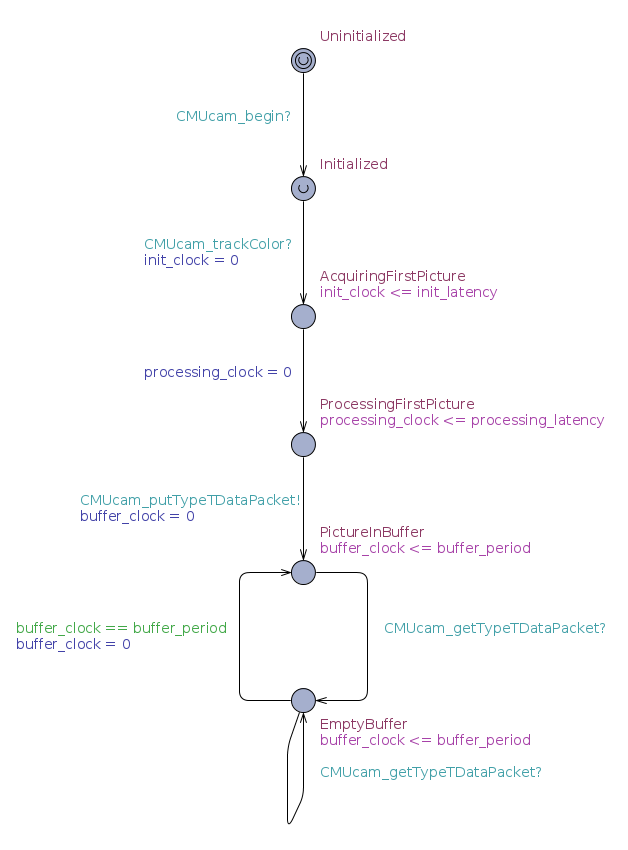
\includegraphics[scale=0.5]{./img/uppaal-camera.png}
      \caption{Modélisation du périphérique {\it Vision Sensor}}
    \end{figure}

    \begin{figure}[!ht]
      \centering
      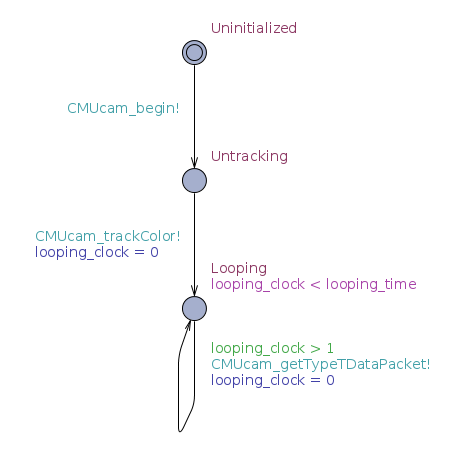
\includegraphics[scale=0.5]{./img/uppaal-loop.png}
      \caption{Modélisation de la tâche {\it Loop}}
    \end{figure}

    \begin{figure}[!ht]
      \centering
      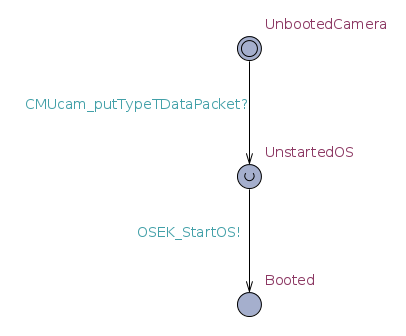
\includegraphics[scale=0.5]{./img/uppaal-boot.png}
      \caption{Modélisation du démarrage du système}
    \end{figure}
    
    \begin{figure}[!ht]
      \centering
      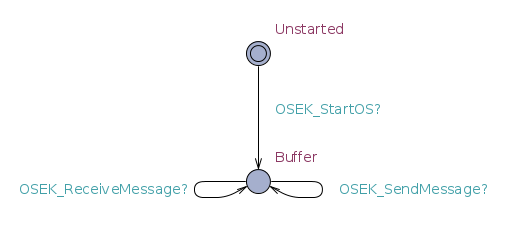
\includegraphics[scale=0.5]{./img/uppaal-buffer.png}
      \caption{Modélisation du buffer du système}
    \end{figure}

    \begin{figure}[!ht]
      \centering
      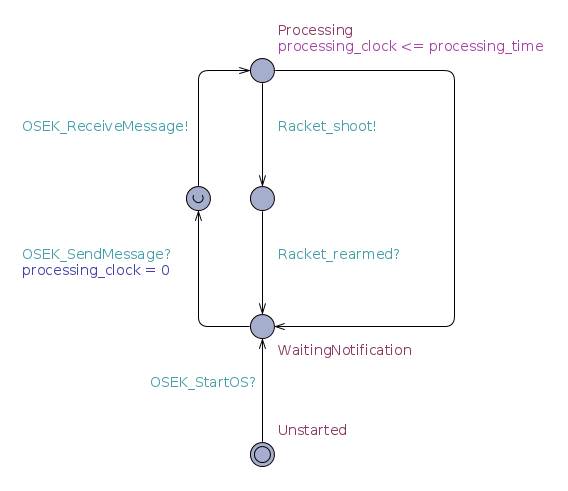
\includegraphics[scale=0.5]{./img/uppaal-task.png}
      \caption{Modélisation de la tâche {\it Control}}
    \end{figure}

    \begin{figure}[!ht]
      \centering
      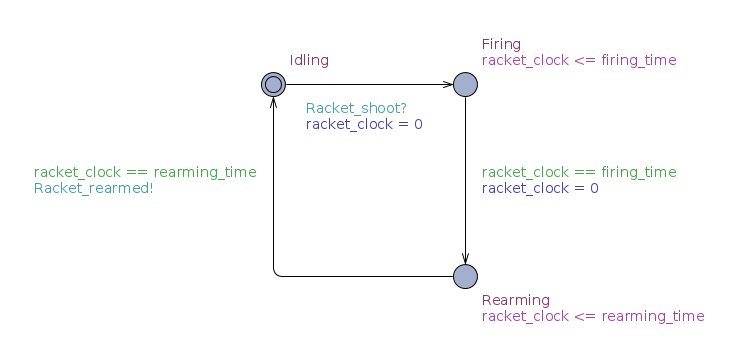
\includegraphics[scale=0.5]{./img/uppaal-racket.png}
      \caption{Modélisation du périphérique {\it Racket}}
    \end{figure}
  
  \FloatBarrier
  \newpage
  \section{Modèle Roméo}
  \label{ann:romeo}

\definecolor{lightgray}{rgb}{.9,.9,.9}

\lstdefinelanguage{cts}{
  keywords={transition, parameters, initially, when, and, do},
  keywordstyle=\bfseries,
  comment=[l]{//},
  commentstyle=\color{purple}
}

\lstset{
  language=cts,
  backgroundcolor=\color{lightgray},
  basicstyle=\footnotesize\ttfamily,
  frame=single,
  rulecolor=\color{black},
  title={Modèle comportemental au format {\it CTS}.}
}

\begin{lstlisting}
  // Declarations:
  parameters 
        init_latency       = 40
    and processing_latency = 60 
    and buffer_period      = 34
    and firing_time        = 5
    and rearming_time      = 7
    and looping_time       = buffer_period
    and polling_time       = 1
    and driver_period      = 50
    and transmission_time  = 2
    and receiving_time     = 4

  initially 
    DEV_camera        := 0,
    DEV_camera_buffer := 0,
    DEV_racket        := 0,
    ARD_loop          := 0,
    ARD_handler       := 0,
    NXT_driver        := 0,
    NXT_driver_period := 0,
    NXT_buffer        := 0,
    NXT_boot          := 0,
    NXT_task          := 0

  // Process DEV_camera:
  transition Camera_Acquiring [0, init_latency]
    when DEV_camera  = 2
    do   DEV_camera := 3

  transition Camera_Updating [buffer_period, buffer_period]
    when DEV_camera  = 4
    do   DEV_camera := 5

  transition Camera_Looping [0, 0]
    when DEV_camera         = 5
    and  DEV_camera_buffer  = 0
    do   DEV_camera        := 4,
         DEV_camera_buffer := 1

  // Process DEV_racket:
  transition Racket_Firing [firing_time, firing_time]
    when DEV_racket  = 1
    do   DEV_racket := 2

  // Processus NXT_driver:
  transition Driver_Activating [driver_period, driver_period]
    when NXT_driver_period  = 1
    do   NXT_driver_period := 0

  // Processus NXT_task:
  transition Task_Processing [0, 0]
    when NXT_task  = 3
    do   NXT_task := 1

  // Synchro CMUcam:
  transition CMUcam_begin
    when ARD_loop    = 0
    and  DEV_camera  = 0
    do   ARD_loop   := 1,
         DEV_camera := 1

  transition CMUcam_trackColor
    when ARD_loop    = 1
    and  DEV_camera  = 1
    do   ARD_loop   := 2,
         DEV_camera := 2

  transition CMUcam_putTypeTDataPacket [0, processing_latency]
    when DEV_camera         = 3
    and  NXT_boot           = 0
    do   DEV_camera        := 4,
         DEV_camera_buffer := 1,
         NXT_boot          := 1

  transition CMUcam_getTypeTDataPacket ]0, looping_time[
    when DEV_camera_buffer  = 1
    and  ARD_loop           = 2
    do   DEV_camera_buffer := 0

  transition CMUcam_getTypeTDataPacket_loop ]0, looping_time[
    when DEV_camera_buffer = 0
    and (DEV_camera = 4 or DEV_camera = 5)
    and  ARD_loop = 2

  // Synchro Driver:
  transition Driver_Busy [0, 0]
    when NXT_driver         = 1
    and  NXT_driver_period  = 0
    and  ARD_handler        = 0
    do   NXT_driver        := 2,
         NXT_driver_period := 1,
         ARD_handler       := 1

  transition Driver_Waiting [receiving_time, receiving_time]
    when NXT_driver   = 4
    and  ARD_handler  = 3
    do   NXT_driver  := 5,
         ARD_handler := 0

  // Synchro Wire:
  transition Wire_onRequest [transmission_time, transmission_time]
    when NXT_driver   = 2
    and  ARD_handler  = 1
    do   NXT_driver  := 3,
         ARD_handler := 2

  transition Wire_write [polling_time, polling_time]
    when ARD_handler  = 2
    and  NXT_driver   = 3
    do   ARD_handler := 3,
         NXT_driver  := 4

  // Synchro OSEK:
  transition OSEK_StartOS [0, 0]
    when NXT_boot    = 1
    and  NXT_buffer  = 0
    and  NXT_driver  = 0
    and  NXT_task    = 0
    do   NXT_boot   := 2,
         NXT_buffer := 1,
         NXT_driver := 1,
         NXT_task   := 1

  transition OSEK_SendMessage [0, 0]
    when NXT_driver  = 5
    and  NXT_buffer  = 1
    and  NXT_task    = 1
    do   NXT_driver := 1,
         NXT_task   := 2

  transition OSEK_ReceiveMessage [0, 0]
    when NXT_task    = 2
    and  NXT_buffer  = 1
    do   NXT_task   := 3

  // Synchro Racket:
  transition Racket_Shoot [0, 0]
    when NXT_task    = 3
    and  DEV_racket  = 0
    do   NXT_task   := 4,
         DEV_racket := 1

  transition Racket_Rearmed [rearming_time, rearming_time]
    when DEV_racket  = 2
    and  NXT_task    = 4
    do   DEV_racket := 0,
         NXT_task   := 1
\end{lstlisting}

